\documentclass{article}
\setlength{\parskip}{5pt} % esp. entre parrafos
\setlength{\parindent}{0pt} % esp. al inicio de un parrafo
\usepackage{amsmath} % mates
\usepackage[sort&compress,numbers]{natbib} % referencias
\usepackage{url} % que las URLs se vean lindos
\usepackage[top=25mm,left=20mm,right=20mm,bottom=25mm]{geometry} % margenes
\usepackage{hyperref} % ligas de URLs
\usepackage{graphicx} % poner figuras
\usepackage[spanish]{babel} % otros idiomas
\usepackage[utf8]{inputenc}
\author{Jesus Alberto Funes Mendoza  \\
Melissa Lizeth Galindo Reyes  \\
Ramón Samuel Blanco Ramirez  \\
Aída Mata Moreno  \\
Miriam Itzel Mata Porras  \\ 
Víctor Adrián Higuera Vázquez} % author
\title{Actividad 3: Generación de pi mediante el método Monte Carlo} % titulo
\date{\today}
\usepackage{float} 
\begin{document} % inicia contenido

\maketitle % cabecera

\begin{abstract} % resumen
El método Montecarlo es un procedimiento donde se escogen una gran variedad de números aleatorios para ser utilizados en operaciones y así tener resultados los cuales serán comparados a lo real y así acercarse mejor a los números más aproximados que explican el fenómeno, para este caso utilizaremos este sistema para cálcular un aproximado al valor de pi y observar su comportamiento de como va cambiando hasta aproximarse al valor deseado en una gráfica.
\end{abstract}

\section{Introducción}\label{intro} % seccion y etiqueta
El método de Monte Carlo tiene un génesis moderno en el trabajo pionero de Stan Ulam y John Von Neumann. Luego de la segunda Guerra Mundial aplicaron distintos métodos de Monte Carlo en simulaciones para el desarrollo de armas termonucleares. Desde entonces y por más de 50 años que se aplicaron estos desarrollos en la investigación y perfeccionamiento de distintos métodos que modelan el transporte de neutrones y radiación gamma con bastante éxito experimental como menciona.

Un método Monte Carlo se puede definir de la siguiente forma:

"Los métodos Monte Carlo son aquéllos en los que las propiedades de las distribuciones de las variables aleatorias son investigadas mediante la simulación de números aleatorios. Estos métodos, dejando a un lado el origen de los datos, son similares a los métodos estadísticos habituales en los cuales las muestras aleatorias se utilizan para realizar inferencias acerca de las poblaciones origen. Generalmente, en su aplicación estadística se utiliza un modelo para simular un fenómeno que contiene algún componente aleatorio. En los métodos Monte Carlo, por otro lado, el objeto de la investigación es un modelo en sí mismo, y se utilizan sucesos aleatorios o pseudoaleatorios para estudiarlo".

El método cobra una especial relevancia las últimas décadas debido a que se produjeron sustanciales y significativos avances respecto a la potencia de los procesadores y las distintas arquitecturas informáticas. Es ampliamente usado en problemas donde obtener un resultado analítico no es posible, o en problemas que contienen demasiada complejidad (como es el caso de la ecuación de transporte de Boltzmann para partículas sin carga)\cite{ff3}.
 



\section{Desarrollo}
\subsection{¿Qué es el método Monte Carlo?}
El termino Monte Carlo se aplica a un conjunto de metodos matemáticos que se empezaron a usar en los 1940s para el desarrollo de armas nucleares en Los Alamos, favorecidos por la aparicion de los ordenadores digitales modernos. Consisten en resolver un ´
problema mediante la invencion de juegos de azar cuyo comportamiento simula algun
fenomeno real gobernado por una distribución de probabilidad (e.g. un proceso físico) o
sirve para realizar un cálculo (e.g. evaluar una integral).
Mas técnicamente, un Monte Carlo es un proceso estocástico numerico, es decir, una 
secuencia de estados cuya evolucion viene determinada por sucesos aleatorios. Recordemos que un suceso aleatorio es un conjunto de resultados que se producen con cierta
probabilidad\cite{ff2}.

\subsection{Modelo de Simulación}

\subsubsection{Generación de números pseudeoaleatorios}
Existen distintos métodos para la generación de números aleatorios, sin embargo, la generación de estos en ordenador parte necesariamente desde una semilla (seed) que es un valor concedido por el usuario. Con esta semilla se genera una única serie de números aleatorios, pudiendo ser replicados a partir de esta. Por esta razón es que se denominan números pseudo aleatorios. La librería Numpy utiliza el algoritmo Mersenne Twistter escribe para la generación de números pseudoaleatorios. Este método particular tiene la cualidad de tener una periodicidad bastante grande en la generación de números\cite{ff2}.

\subsubsection{Métodos de estimación de pi}
Se propone estimar el número de pi con el siguiente modelo: Consideramos un cuadrado de lado L, con una circunferencia en su interior de radio L. La relación de áreas se da en Ec. 19\cite{ff2}:


\begin{figure}[H] % figura
    \centering
    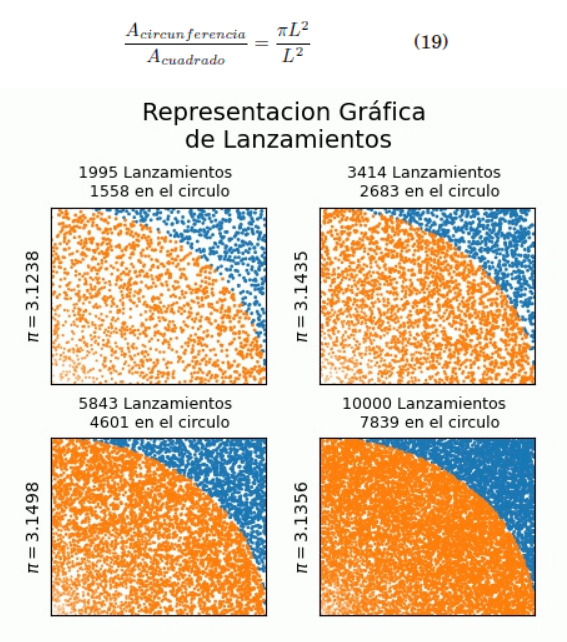
\includegraphics[width=80mm]{imagen1.png} % archivo
    \caption{Representación gráfica de la estimación de pi mediante el lanzamiento aleatorio de puntos. Mientras mayor sea el número de lanzamientos las áreas son más definidas\cite{ff2}}
    \label{grafica:trece}
\end{figure}

\section{Simulación}
En está sección observaremos como fue escrito el programa utilizado en Python, también es necesario aclarar que en caso de que algún compilador no funcione, simplemtente es necesario dirigirse a la tecla windows y escribir 'cmd', dentro de esta ventana que abra, hay que escribir 'pip install' y después la libreía que no este descargada en el ordenador.


\begin{figure}[H] % figura
    \centering
    \includegraphics[width=80mm]{código_1.jpeg} % archivo
    \centering
    \includegraphics[width=80mm]{código_2.jpeg} % archivo
    \caption{Código completo para la programación de las gráficas de Montecarlo para obtener un valor cercano a pi con números aleatorios, estos códigos divididos en secciones para disntinguir mejor donde se realizan cálculos o la gráfica o las librerías, entre otras.}
    \label{grafica:trece}
\end{figure}

\subsection{Resultados}
A continuación se mostrarán las gráficas que obtuvimos donde destacará el acercamiento al valor de pi desde un número probablemente muy diferente como inicio.

\begin{figure}[H] % figura
    \centering
    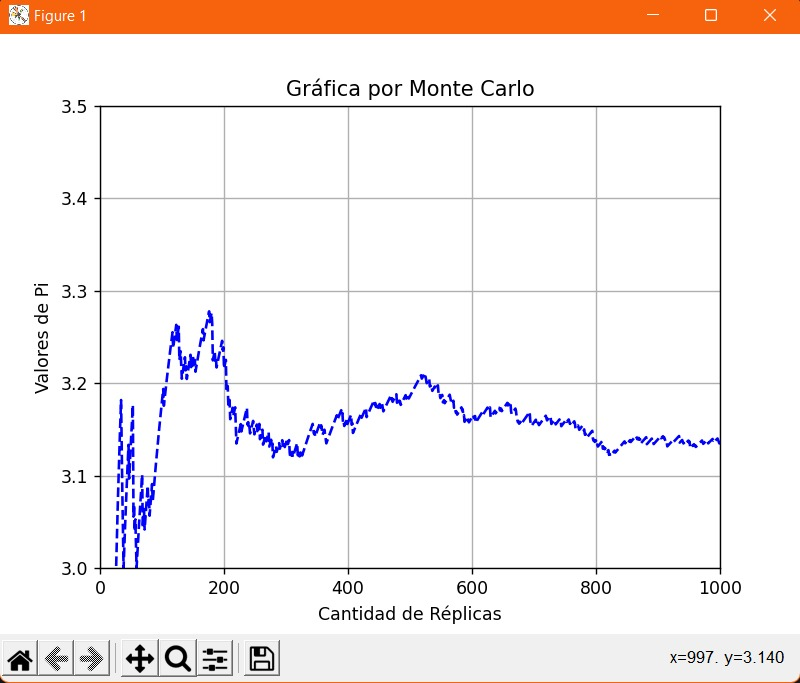
\includegraphics[width=80mm]{60.jpeg} % archivo
    \centering
    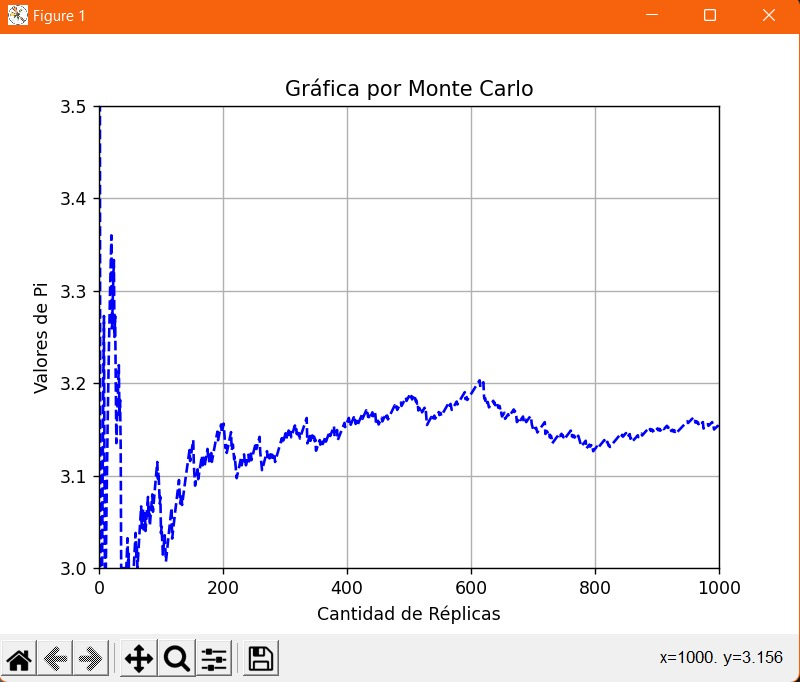
\includegraphics[width=80mm]{125.jpeg} % archivo
    \centering
    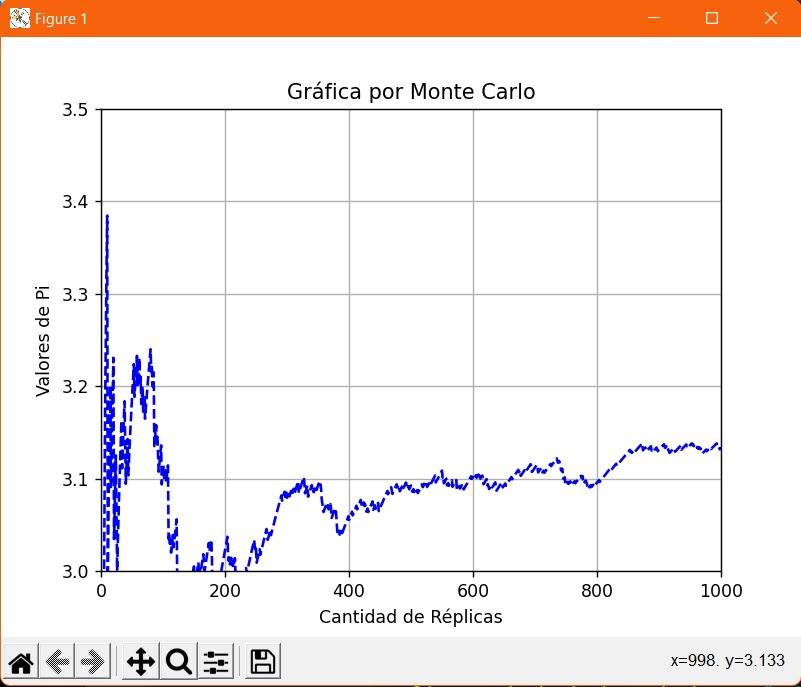
\includegraphics[width=80mm]{250.jpeg} % archivo
    \centering
    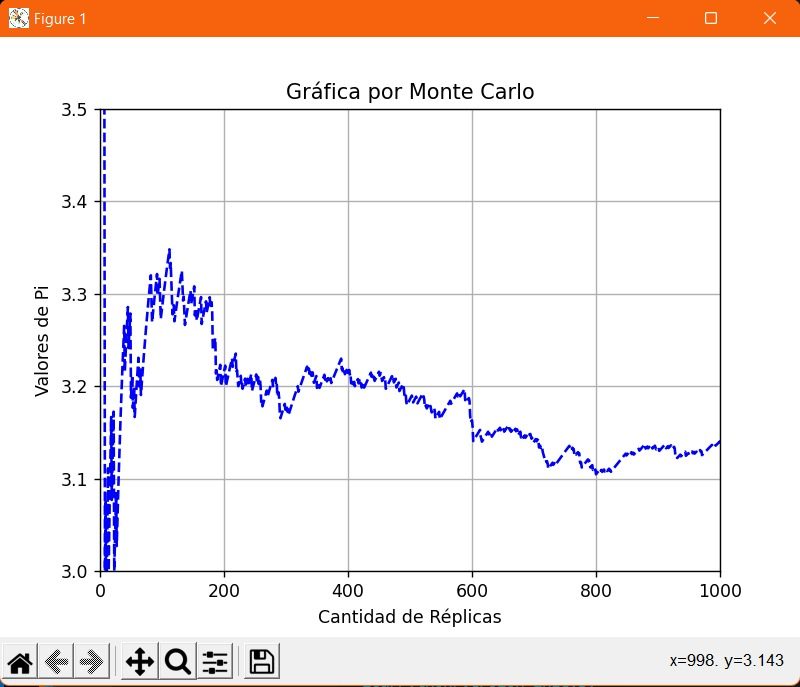
\includegraphics[width=80mm]{500.jpeg} % archivo
    \centering
    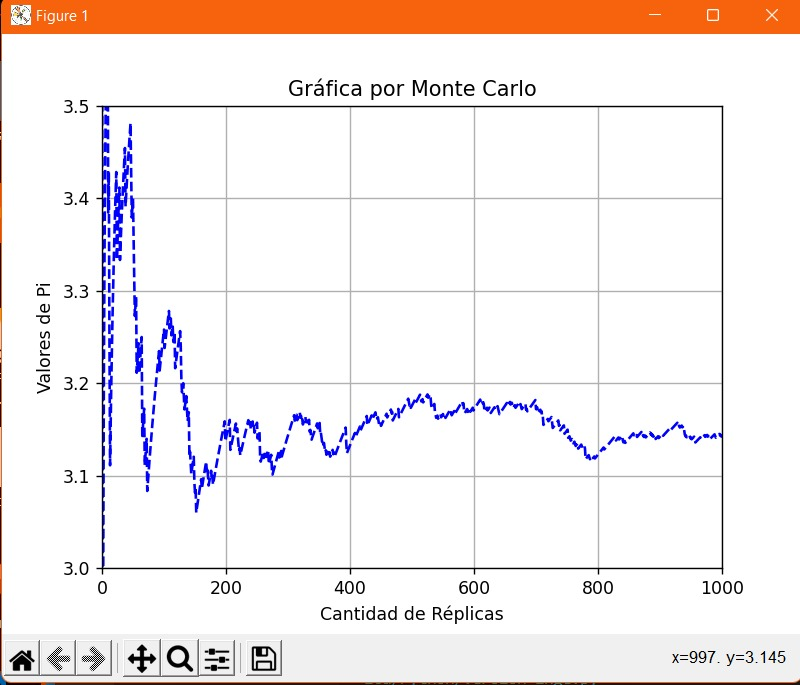
\includegraphics[width=80mm]{1000.jpeg} % archivo
    \centering
    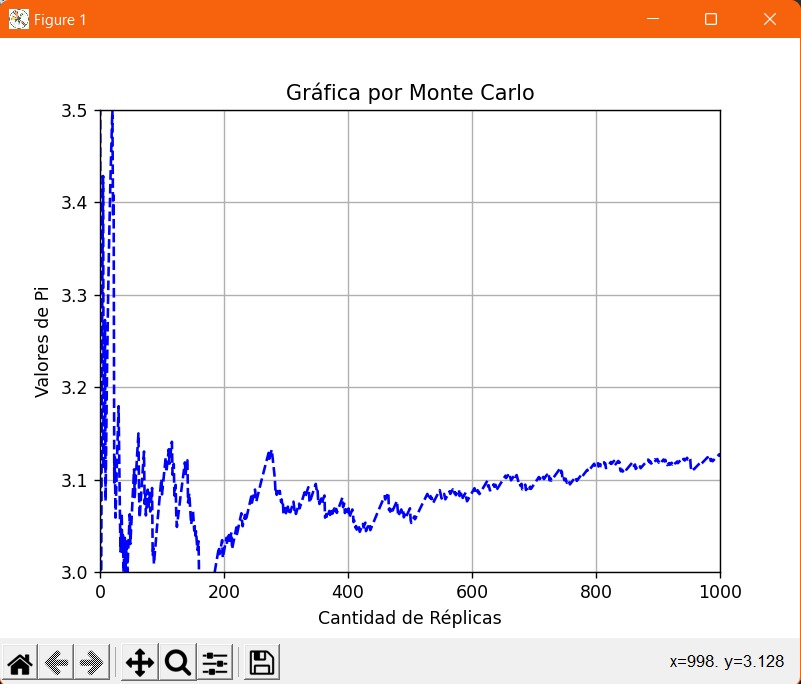
\includegraphics[width=80mm]{5000.jpeg} % archivo
    \label{grafica:trece}
\end{figure}

\begin{figure}[H] % figura
    \centering
    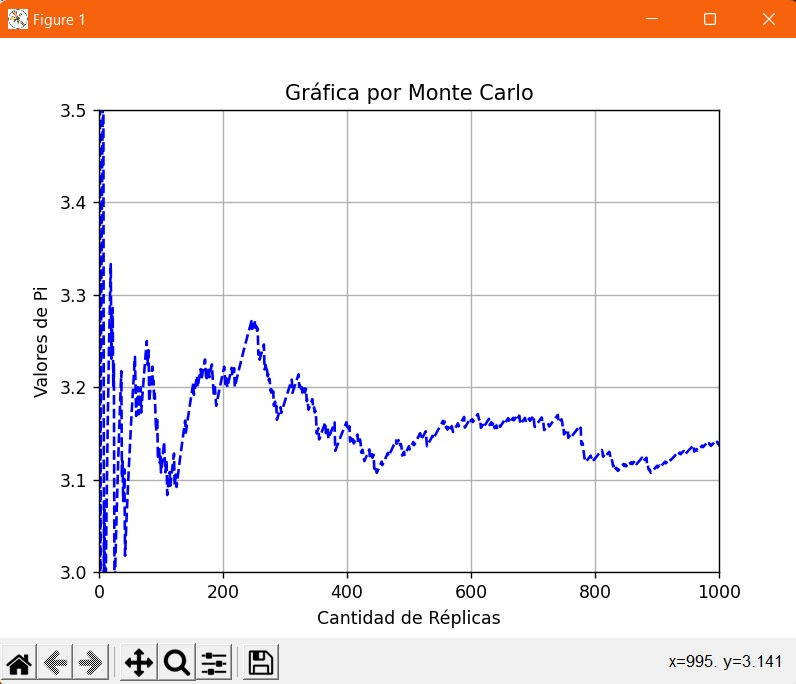
\includegraphics[width=80mm]{10000.jpeg} % archivo
    \caption{Estos resultados varían en cuanto al número de réplicas que se utilizo en cada uno, empezando de izquierda y yendo a la derecha va de: 60, 125, 250, 500, 1000 y 10000 réplicas}
\end{figure}


\section{Conclusiones}
Al inicio de esta actividad pensamos que no nos tomaría mucho tiempo, pero casi desde la instalación del programa nos faltó poner algunas librerías, ningún código compilaba y consideramos que como futuros ingenieros en mecatrónica desde los primeros semestres se nos debió de haber inculcado más la programación para no batallar en semestres avanzados como este al momento de programar, pero este tipo de actividades nos ayuda a mejorar en el área de programación esperando ir mejorando conforme cada semestre. 

\bibliography{bib}
\bibliographystyle{plainnat}

\end{document}

